\documentclass{standalone}

\usepackage[latin1]{inputenc}
\usepackage{amsmath}
\usepackage{amssymb}
\usepackage{amsthm}

\usepackage{tikz}
\usetikzlibrary{arrows}

%% generates a tightly fitting border around the work
%\usepackage[active,tightpage]{preview}
%\PreviewEnvironment{tikzpicture}
%\setlength\PreviewBorder{0.5mm}
%%\renewcommand\PreviewBbAdjust{-\PreviewBorder 1mm -1.15mm -0.85mm}

\usepackage{color}

%\pagestyle{empty}

\begin{document}

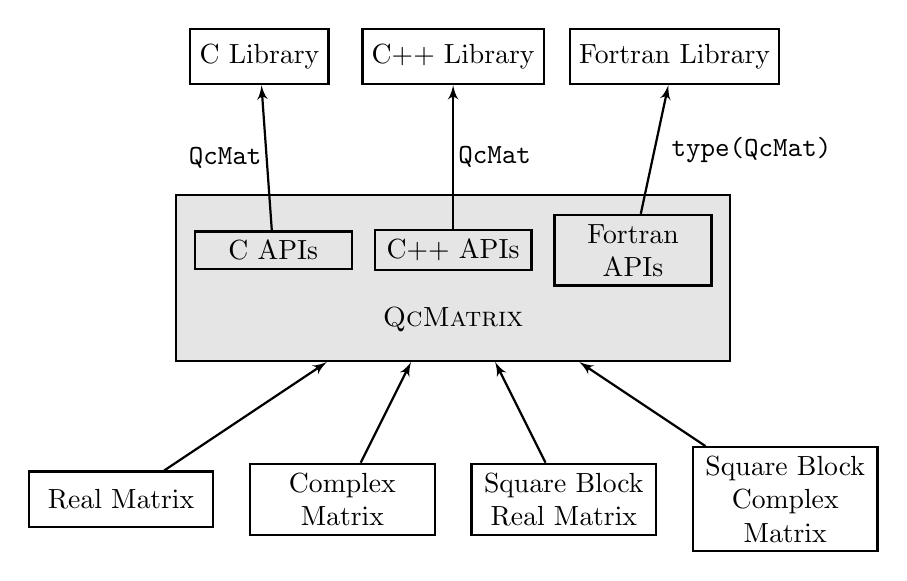
\begin{tikzpicture}[thick, node distance=80]
  \node[color=black, rectangle, draw, text badly centered, sharp corners, minimum height=60, % 
        minimum width=200, fill=black!10] (QcMatrix) {~};
  \node[below of=QcMatrix, yshift=65] {\textsc{QcMatrix}};
  % APIs
  \node[color=black, rectangle, draw, text badly centered, sharp corners, minimum height=2, %
        text width=50, xshift=-65, yshift=-70, above of=QcMatrix] (CAPIs) {C APIs};
  \node[color=black, rectangle, draw, text badly centered, sharp corners, minimum height=2, %
        text width=50, yshift=-70, above of=QcMatrix] (CppAPIs) {C++ APIs};
  \node[color=black, rectangle, draw, text badly centered, sharp corners, minimum height=2, %
        text width=50, xshift=65, yshift=-70, above of=QcMatrix] (FAPIs) {Fortran APIs};
  % application libraries
  \node[color=black, rectangle, draw, text badly centered, sharp corners, minimum height=20, %
        above of=QcMatrix, xshift=-70] (LibAppC) {C Library};
  \node[color=black, rectangle, draw, text badly centered, sharp corners, minimum height=20, %
        above of=QcMatrix] (LibAppCpp) {C++ Library};
  \node[color=black, rectangle, draw, text badly centered, sharp corners, minimum height=20, %
        above of=QcMatrix, xshift=80] (LibAppF) {Fortran Library};
  % different matrices
  \node[color=black, rectangle, draw, text badly centered, sharp corners, minimum height=20, %
        text width=60, below of=QcMatrix, xshift=-120] (RealMat) {Real Matrix};
  \node[color=black, rectangle, draw, text badly centered, sharp corners, minimum height=20, %
        text width=60, below of=QcMatrix, xshift=-40] (CmplxMat) {Complex Matrix};
  \node[color=black, rectangle, draw, text badly centered, sharp corners, minimum height=20, %
        text width=60, below of=QcMatrix, xshift=40] (RealBlock) {Square Block Real Matrix};
 \node[color=black, rectangle, draw, text badly centered, sharp corners, minimum height=20, %
        text width=60, below of=QcMatrix, xshift=120] (CmplxBlock) {Square Block Complex Matrix};
  \draw [color=black, -latex'] (CAPIs)edge node[midway, xshift=-15]{\texttt{QcMat}}(LibAppC);
  \draw [color=black, -latex'] (CppAPIs)edge node[midway, xshift=15]{\texttt{QcMat}}(LibAppCpp);
  \draw [color=black, -latex'] (FAPIs)edge node[midway, xshift=35]{\texttt{type(QcMat)}}(LibAppF);
  \draw [color=black, -latex'] (RealMat)--(QcMatrix);
  \draw [color=black, -latex'] (CmplxMat)--(QcMatrix);
  \draw [color=black, -latex'] (RealBlock)--(QcMatrix);
  \draw [color=black, -latex'] (CmplxBlock)--(QcMatrix);
\end{tikzpicture}

\end{document}
